\chapter{Benchmarking ST against Texas Instruments}
\label{chap:vs-ti}

\section*{Introduction}

The TI work forms the second extended campaign. It moves beyond the pilot's USB-only scope
and the GD32 campaign by combining source-level driver analysis, matched bare-metal
projects, and FreeRTOS scenarios. Its conclusions must therefore remain separate from the
earlier campaign designs rather than being merged into a single cross-vendor ranking.

Texas Instruments (TI) is one of the world's largest semiconductor manufacturers, with a
broad portfolio of embedded processors and microcontrollers~\cite{ti-about}. Its MSPM0 and
MSPM3 families, built around Arm Cortex-M0+ and Cortex-M33 cores respectively, target
cost-sensitive and mixed-signal applications with a strong emphasis on analog
integration~\cite{ti-mspm33-product}. Unlike GigaDevice, which competes primarily on
pin-compatibility, TI competes on a fundamentally different SDK architecture: a
SysConfig-centric, unified serial peripheral model and a single-layer driver library
(driverlib) rather than the dual HAL/LL approach used by STMicroelectronics.

This chapter presents the ST-versus-TI comparison in two complementary phases. The first is a
comprehensive \textbf{static analysis} of the low-level driver layers of both SDKs. Unlike the
runtime-focused benchmarks in Chapter~\ref{chap:vs-gd32}, this analysis examines source-code
quality and SDK breadth without executing firmware on hardware. The second phase combines
twelve low-level-driver scenarios with a FreeRTOS middleware benchmark covering basic,
cooperative, and preemptive processing. We compare the
STM32CubeC5 Low-Layer (LL) drivers~\cite{stm32cubec5-sw} against the TI MSPM33 SDK
driverlib~\cite{ti-mspm33-sdk} across seven quality dimensions --- lines of code,
documentation coverage, code duplication, cyclomatic complexity, API surface design,
MISRA~C:2012 compliance, and security (CWE analysis). For the scope definition, we also
map the SDK coverage in terms of peripheral drivers, middleware, cryptographic algorithms,
and communication protocols, identifying what each vendor offers exclusively.

All measurements were produced by automated scripts using
\texttt{cloc}~\cite{cloc-tool}, \texttt{cppcheck}~\cite{cppcheck-tool} (with its
\texttt{--addon=misra} and \texttt{--addon=cert} modes),
\texttt{lizard}~\cite{lizard-tool} for cyclomatic complexity, and
\texttt{jscpd}~\cite{jscpd-tool} for duplication detection.

% ====================================================================
\section{Hardware platforms}
\label{sec:ti-boards}

The analysis in this chapter targets driver code for two boards hosting comparable
Cortex-M33 parts. Table~\ref{tab:ti-board-comparison} summarises their key characteristics.

\begin{table}[H]
\centering
\caption{Board and MCU comparison --- STM32C5A3 vs.\ MSPM33C321A~\cite{stm32c5a3-product,stm32-nucleo-c5a3,ti-mspm33-ds,ti-launchpad}.}
\label{tab:ti-board-comparison}
\begin{tabularx}{\textwidth}{@{}l >{\raggedright\arraybackslash}X >{\raggedright\arraybackslash}X@{}}
\toprule
\textbf{Feature} & \textbf{STM32C5A3 (NUCLEO-C5A3ZG)} & \textbf{MSPM33C321A (LP-MSPM33C321A)} \\
\midrule
Core & Arm Cortex-M33 (FPU, DSP, MPU) & Arm Cortex-M33 (FPU, DSP, TrustZone) \\
Max frequency & 144\,MHz & 160\,MHz \\
Flash & 1\,MB (ECC, dual-bank) & 1\,MB (ECC, dual-bank, address swap) \\
SRAM & 256\,KB (128\,KB with ECC) & 256\,KB (ECC) \\
ADC & 3 $\times$ 12-bit, 4.5\,MSPS & 2 $\times$ 12-bit, 9.4\,MSPS \\
DAC & 1 $\times$ 12-bit & 2 $\times$ 8-bit \\
CAN & 2 $\times$ FDCAN & 2 $\times$ CAN\,FD \\
USB & USB\,2.0 FS (Host/Device/DRD) & --- \\
Ethernet & Yes (MAC with DMA) & --- \\
I3C & Yes & --- \\
Debug probe & ST-LINK & XDS110 (EnergyTrace) \\
\bottomrule
\end{tabularx}
\end{table}

Both parts share the same core architecture and identical flash/RAM capacities, which makes
the comparison fair at the silicon level. The STM32C5A3 offers broader connectivity (USB,
Ethernet, I3C), while the MSPM33C321A favours higher analog bandwidth (9.4\,MSPS ADC) and
provides TrustZone support~\cite{ti-mspm33-ds,stm32c5a3-product}.

% ====================================================================
\section{Static analysis of the driver layer}
\label{sec:ti-static-analysis}

This section compares the LL driver layer of STM32CubeC5 against the driverlib of the
MSPM33 SDK. The LL layer was chosen for ST because it is the closest architectural
equivalent to TI's driverlib: both are thin, inline-heavy abstractions over peripheral
registers, designed for performance-critical code. We analyse seven complementary
dimensions.

% --------------------------------------------------------------------
\subsection{Scope and methodology}
\label{subsec:ti-scope}

The analysis targets the following source sets:

\begin{itemize}
  \item \textbf{ST:} all 33 header files in
        \texttt{stm32c5xx\_drivers/ll/} (the LL layer of STM32CubeC5).
  \item \textbf{TI:} all 85 source and header files in
        \texttt{source/ti/driverlib/} and its \texttt{m33/} subdirectory
        (the driverlib of MSPM33 SDK v1.03.00.01).
\end{itemize}

Both sets were analysed on the same workstation under identical tool configurations. The
tools and their roles are:

\begin{itemize}
  \item \textbf{cloc} v2.08~\cite{cloc-tool} --- counts blank, comment, and code lines per
        language and file.
  \item \textbf{lizard}~\cite{lizard-tool} --- computes cyclomatic complexity, number of
        parameters, and token count per function.
  \item \textbf{cppcheck} v2.x~\cite{cppcheck-tool} --- runs MISRA~C:2012 addon
        (\texttt{--addon=misra}) and CWE/CERT checks.
  \item \textbf{jscpd}~\cite{jscpd-tool} --- detects copy-pasted code blocks (duplication).
      \item A custom Python analysis script extracts API surface
        metrics (public/static/inline functions, macros, enums, naming patterns, parameter
        distributions) and documentation coverage (Doxygen blocks, \texttt{@brief},
        \texttt{@param}, \texttt{@return} tags, file headers).
\end{itemize}

% --------------------------------------------------------------------
\subsection{Lines of code}
\label{subsec:ti-loc}

Table~\ref{tab:ti-loc} presents the line-count breakdown for each SDK's driver layer.

\begin{table}[H]
\centering
\caption{Lines-of-code comparison --- ST LL vs.\ TI driverlib.}
\label{tab:ti-loc}
\begin{tabular}{l r r}
\toprule
\textbf{Metric} & \textbf{ST (LL)} & \textbf{TI (driverlib)} \\
\midrule
Source files      &        33 &        85 \\
Blank lines       &     5\,744 &     8\,747 \\
Comment lines     &    57\,649 &    45\,763 \\
Code lines        &    22\,292 &    27\,972 \\
\midrule
Total lines       &    85\,685 &    82\,482 \\
Comment-to-code ratio & 2.59 & 1.64 \\
\bottomrule
\end{tabular}
\end{table}

ST delivers its LL layer in 33 header-only files containing 22\,292 lines of code, while
TI spreads its driverlib across 85 files (both \texttt{.c} and \texttt{.h}) with
27\,972 code lines. Despite having 25\% more code, TI's total line count is slightly
lower because ST invests significantly more in inline comments: 57\,649 comment lines
versus 45\,763, yielding a comment-to-code ratio of 2.59 for ST compared with 1.64 for TI.
This difference reflects ST's header-only, fully-documented inline function strategy, where
each function carries extensive Doxygen annotations embedded alongside the implementation.

% --------------------------------------------------------------------
\subsection{Documentation coverage}
\label{subsec:ti-doc}

We measured documentation quality through Doxygen tag extraction.
Table~\ref{tab:ti-doc} summarises the results.

\begin{table}[H]
\centering
\caption{Documentation coverage --- ST LL vs.\ TI driverlib.}
\label{tab:ti-doc}
\begin{tabular}{l r r}
\toprule
\textbf{Metric} & \textbf{ST (LL)} & \textbf{TI (driverlib)} \\
\midrule
Total functions         &   3\,713 &   3\,056 \\
Documented functions    &   3\,613 &   2\,525 \\
\textbf{Doc.\ coverage} & \textbf{97.3\,\%} & \textbf{82.6\,\%} \\
\midrule
Doxygen blocks          &   5\,967 &   3\,357 \\
\texttt{@brief} tags    &   3\,826 &   5\,568 \\
\texttt{@param} tags    &   4\,440 &   3\,970 \\
\texttt{@return} tags   &   1\,705 &   2\,172 \\
File headers            &      33  &      85  \\
Inline comments         &       0  &     283  \\
\bottomrule
\end{tabular}
\end{table}

ST achieves 97.3\% function-level documentation coverage, leaving only 100 undocumented
functions. TI reaches 82.6\%, with 531 undocumented functions --- mostly in \texttt{.c}
implementation files, where TI concentrates complex logic (e.g.\ flash controller
operations, PLL configuration) without per-function Doxygen blocks. This architectural
choice is deliberate: TI documents the \emph{header} API thoroughly but omits Doxygen in
\texttt{.c} bodies, whereas ST's header-only approach means every function definition is
also its documented declaration.

Interestingly, TI uses more \texttt{@brief} tags (5\,568 vs.\ 3\,826) and more
\texttt{@return} tags (2\,172 vs.\ 1\,705), suggesting that when TI does document a
function, it tends to be descriptive about purpose and return values. ST, however, produces
78\% more Doxygen blocks overall (5\,967 vs.\ 3\,357), reflecting its higher raw volume of
documented entities.

% --------------------------------------------------------------------
\subsection{Code duplication}
\label{subsec:ti-dup}

Table~\ref{tab:ti-dup} presents the duplication metrics.

\begin{table}[H]
\centering
\caption{Code duplication --- ST LL vs.\ TI driverlib.}
\label{tab:ti-dup}
\begin{tabular}{l r r}
\toprule
\textbf{Metric} & \textbf{ST (LL)} & \textbf{TI (driverlib)} \\
\midrule
Total lines analysed     &    85\,685 &    82\,403 \\
Code lines               &    10\,461 &    18\,008 \\
Duplicate blocks         &        71 &       414 \\
Duplicate lines          &       229 &     1\,306 \\
\textbf{Duplication \%}  & \textbf{2.19\,\%} & \textbf{7.25\,\%} \\
\midrule
Same-file clones         &        71 &       338 \\
Cross-file clones        &         0 &        76 \\
\bottomrule
\end{tabular}
\end{table}

TI's driver layer exhibits 3.3$\times$ more duplication than ST's (7.25\% vs.\ 2.19\%).
All 71 duplicate blocks in ST occur within the same file, typically in symmetric
getter/setter pairs for multi-channel peripherals (e.g.\ ADC rank configuration).
TI, by contrast, has 76 cross-file clones --- code that is structurally identical across
different peripheral modules. This pattern arises from TI's UniComm architecture, where
\texttt{dl\_unicommuart.h}, \texttt{dl\_unicommspi.h}, and \texttt{dl\_unicommi2cc.h}
share a common General Serial Controller (GSC) base but replicate similar interrupt-handling
and configuration boilerplate in each specialisation.

The higher duplication in TI is not inherently a quality defect --- it reflects a design
choice that trades some code reuse for peripheral-specific readability. However, from a
maintenance perspective, ST's lower duplication means fewer locations to update when fixing
a bug or adapting to silicon errata.

% --------------------------------------------------------------------
\subsection{Cyclomatic complexity}
\label{subsec:ti-complexity}

Cyclomatic complexity (CC) measures the number of linearly independent paths through a
function; higher values indicate more decision branches and, consequently, harder-to-test
code~\cite{lizard-tool}. We ran Lizard on every function in both driver sets and
summarise the results in Table~\ref{tab:ti-complexity}.

\begin{table}[H]
\centering
\caption{Cyclomatic complexity comparison --- ST LL vs.\ TI driverlib.}
\label{tab:ti-complexity}
\begin{tabular}{l r r}
\toprule
\textbf{Metric} & \textbf{ST (LL)} & \textbf{TI (driverlib)} \\
\midrule
Analysed functions       &    3\,542 &    2\,539 \\
Mean CC                  &      4.44 &      7.35 \\
Median CC                &         4 &         5 \\
Maximum CC               &        49 &       141 \\
\midrule
Functions with CC $>$ 10 &    44 \scriptsize(1.2\,\%) &   335 \scriptsize(13.2\,\%) \\
Functions with CC $>$ 20 &    12 \scriptsize(0.3\,\%) &    97 \scriptsize(3.8\,\%) \\
\bottomrule
\end{tabular}
\end{table}

Under the study's declared CC\,=\,10 review threshold, ST's analysed driver code is
flatter: the average function has fewer than five decision points, and 1.2\,\% of functions
exceed that threshold. The maximum (CC\,=\,49) occurs in a temperature-calculation
helper (\texttt{LL\_ADC\_CALC\_TEMPERATURE}) that contains a long chain of calibration
look-ups.

TI's SDK shows a heavier tail: 13.2\,\% of its functions exceed CC\,=\,10, with a peak of
141 in a single function. Many of these high-complexity functions reside in the UniComm
serial-controller layer, where a large \texttt{switch} dispatches configuration variants
for UART, SPI, and I\textsuperscript{2}C through a shared code path. While this design
consolidates peripheral logic, it concentrates branching in ways that complicate unit testing
and formal verification.

Under this metric, ST's analysed source set contains fewer functions above the declared
review threshold. The result does not by itself establish maintainability or safety.

% --------------------------------------------------------------------
\subsection{API surface}
\label{subsec:ti-api}

Table~\ref{tab:ti-api} compares the API design characteristics.

\begin{table}[H]
\centering
\caption{API surface comparison --- ST LL vs.\ TI driverlib.}
\label{tab:ti-api}
\begin{tabular}{l r r}
\toprule
\textbf{Metric} & \textbf{ST (LL)} & \textbf{TI (driverlib)} \\
\midrule
Public functions         &    3\,543 &    2\,500 \\
Static functions         &         1 &        42 \\
Inline functions         &    3\,543 &    2\,032 \\
Functional macros        &       194 &        27 \\
Constant macros          &     3\,993 &    3\,271 \\
Enums                    &         1 &       361 \\
Typedefs                 &         0 &       470 \\
\midrule
Avg.\ parameters/func.  &      1.17 &      1.69 \\
Max parameters           &         8 &         8 \\
\texttt{extern "C"} guards &    33 &        43 \\
Include guards           &        33 &         0 \\
\bottomrule
\end{tabular}
\end{table}

The two APIs reflect fundamentally different design philosophies:

\begin{itemize}
  \item \textbf{ST LL} exposes 3\,543 public functions, \emph{all} of which are
        \texttt{\_\_STATIC\_INLINE}. The API is almost entirely composed of one-parameter
      getters and status queries.
        Type safety relies on constant macros rather than enums. The naming convention
        follows the \texttt{LL\_PERIPHERAL\_Action} pattern consistently across all 33
        files.
  \item \textbf{TI driverlib} exposes 2\,500 public functions, of which 2\,032 are inline
        (81\%). It makes heavier use of enums (361 enum types) and typedefs (470) for
        configuration parameters, which improves type safety and IDE autocompletion at the
        cost of a more complex type graph. The naming convention follows
        \texttt{DL\_Peripheral\_Action} uniformly. Functions tend to take more parameters
        on average (1.69 vs.\ 1.17), reflecting a more configuration-object-oriented
        style where a single call sets multiple related fields.
\end{itemize}

ST's 194 functional macros versus TI's 27 show that the analysed ST source set uses more
preprocessor computation in places such as register-offset calculations and bit-field
assembly. Inline functions permit stronger compile-time type checking than function-like
macros, but this study did not compare generated machine code or debugging productivity.

% --------------------------------------------------------------------
\subsection{MISRA~C:2012 static-analysis findings}
\label{subsec:ti-misra}

Both SDKs were analysed using \texttt{cppcheck} with the MISRA~C:2012
addon~\cite{misra-c2012}. Table~\ref{tab:ti-misra} presents the per-rule breakdown.

\begin{table}[H]
\centering
\caption{Cppcheck MISRA-addon findings --- ST LL vs.\ TI driverlib.}
\label{tab:ti-misra}
\begin{tabular}{l l r r}
\toprule
\textbf{Rule} & \textbf{Description} & \textbf{ST} & \textbf{TI} \\
\midrule
17.3 & Function declared implicitly       & 3\,541 &  281 \\
11.4 & Conversion between pointer and integer & 84 &    4 \\
10.6 & Composite expression assigned to wider type & 29 & --- \\
20.7 & Macro parameter not enclosed in parentheses & 21 & --- \\
7.3  & Lower-case ``l'' suffix on literal  &    18 & --- \\
10.4 & Incompatible essential types in operation & --- & 67 \\
12.1 & Precedence of operators unclear     & --- &   52 \\
18.4 & Pointer arithmetic                  & --- &   76 \\
15.5 & Multiple return statements          &     4 &   14 \\
10.1 & Operands of inappropriate essential type & --- & 13 \\
3.1  & Comment contains nested comment     & --- &   11 \\
Other & Various minor rules                &    6 &   33 \\
\midrule
\textbf{Total} & & \textbf{3\,703} & \textbf{551} \\
\bottomrule
\end{tabular}
\end{table}

\subsubsection*{Interpretation}
The raw Cppcheck output reports 3\,703 findings for ST and 551 for TI. Rule~17.3 accounts
for 3\,541 ST findings and 281 TI findings. The current analysis attributes many ST
findings to processing header-only inline code in isolation, but the original preprocessing
inputs and a compilation-database rerun are not available with the report artifacts. We
therefore present exclusion of Rule~17.3 only as a sensitivity calculation, not as proof
that every such finding is a false positive. Under that exclusion, the counts are 162 for
ST and 270 for TI. These are tool-reported findings for the analysed source sets and do not
constitute MISRA certification or a complete compliance assessment.

The remaining findings also require source-level review. Rule~11.4 includes casts between
integers and peripheral base-address pointers, a common low-level-driver pattern, while TI's
reported findings span rules concerning pointer arithmetic, essential types, and operator
precedence. Counts alone do not establish the severity or correctness impact of these
patterns.

\subsubsection*{Security analysis (CWE)}
Both driver layers returned \textbf{zero CWE findings} from \texttt{cppcheck}'s CERT/CWE
checker. Neither SDK contains patterns flagged as common weakness enumerations, which is
expected for thin, register-level driver code that performs no dynamic allocation, string
handling, or network I/O.

% ====================================================================
\section{SDK coverage comparison}
\label{sec:ti-sdk-coverage}

Beyond driver-layer quality, the breadth of a selected SDK release --- how many peripherals, middleware
stacks, and communication protocols it supports out of the box --- determines the
development effort required for a real product. We inventoried the selected STM32CubeC5
and MSPM33 SDK source sets file by file and identified features present on only one side
within those releases~\cite{stm32cubec5-sw,ti-mspm33-sdk}.

% --------------------------------------------------------------------
\subsection{Peripheral driver coverage}
\label{subsec:ti-periph-gaps}

Table~\ref{tab:ti-periph-exclusive} lists the peripheral drivers present in only one
SDK.\footnote{For brevity, only a representative subset of ST's 25 exclusive drivers is
shown; the full list is available in the analysis output.}

\begin{table}[H]
\centering
\caption{Exclusive peripheral drivers in the selected SDK releases~\cite{stm32cubec5-sw,ti-mspm33-sdk}.}
\label{tab:ti-periph-exclusive}
\begin{tabular}{l p{5.5cm} l}
\toprule
\textbf{Vendor} & \textbf{Driver} & \textbf{Capability} \\
\midrule
\multicolumn{3}{l}{\textit{ST-exclusive (25 drivers)}} \\
ST & CORDIC accelerator              & HW trigonometric/hyperbolic math \\
ST & DAC (12-bit)                    & Full DAC peripheral \\
ST & Ethernet MAC                    & On-chip networking \\
ST & USB Host / Device / DRD         & Full USB stack support \\
ST & I3C controller                  & Next-gen I3C bus \\
ST & HASH accelerator (SHA)          & HW SHA-1/SHA-256 \\
ST & OPAMP                           & On-chip operational amplifier \\
ST & ICACHE controller               & Configurable instruction cache \\
ST & XSPI (Octo/Quad-SPI)           & Advanced memory-mapped SPI \\
ST & LPUART, USART, SmartCard, SMBus & Extended serial protocols \\
\midrule
\multicolumn{3}{l}{\textit{TI-exclusive (16 drivers)}} \\
TI & High-Speed ADC (HSADC)          & Dedicated 9.4\,MSPS ADC block \\
TI & General Serial Controller (GSC) & Unified serial engine \\
TI & UniComm (I2C/SPI/UART)          & Configurable serial block \\
TI & Signal Processing Subsystem     & On-chip analog processing \\
TI & Low-Frequency Subsystem (LFSS)  & Unified RTC + tamper + scratchpad \\
TI & Key Store Controller            & HW key management \\
TI & Error Action Module             & HW automatic fault handling \\
TI & UART extend (IrDA, Manchester)  & Extended UART modes \\
\bottomrule
\end{tabular}
\end{table}

ST leads with 25 exclusive peripheral drivers to TI's 16. The most significant gaps are
in connectivity: ST offers USB, Ethernet, and I3C, which are entirely absent from the
MSPM33C321A. TI compensates with stronger analog integration (high-speed ADC, signal
processing subsystem) and a unified serial architecture that consolidates UART, SPI, and
I2C into a single configurable peripheral.

% --------------------------------------------------------------------
\subsection{Middleware coverage}
\label{subsec:ti-mw-gaps}

Table~\ref{tab:ti-mw-exclusive} compares the middleware stacks.

\begin{table}[H]
\centering
\caption{Exclusive middleware in the selected SDK releases~\cite{stm32cubec5-sw,ti-mspm33-sdk}.}
\label{tab:ti-mw-exclusive}
\begin{tabular}{l l p{6cm}}
\toprule
\textbf{Vendor} & \textbf{Middleware} & \textbf{Purpose} \\
\midrule
ST & FileX              & FAT-compatible embedded file system \\
ST & LevelX             & Flash wear-leveling (NAND/NOR) \\
ST & LwIP               & Lightweight TCP/IP stack \\
ST & USBX               & USB device/host class drivers \\
ST & mbedTLS             & TLS/SSL library (TLS~1.2/1.3) \\
ST & Open Bootloader     & Multi-interface bootloader \\
ST & stFCF               & Security provisioning framework \\
ST & stCryptoLib          & Comprehensive crypto library \\
\midrule
TI & Edge AI             & On-device ML inference \\
TI & LVGL                & Embedded graphics/GUI library \\
TI & LIN Bus             & Automotive LIN protocol \\
TI & DALI                & Smart lighting protocol \\
TI & IQmath              & Fixed-point DSP math library \\
TI & Post-Quantum Crypto & ML-DSA (Dilithium) signatures \\
TI & Curve25519          & Modern elliptic curve crypto \\
\bottomrule
\end{tabular}
\end{table}

ST provides 8 exclusive middleware components focused on connectivity (USB, Ethernet/IP,
file system) and security (TLS, crypto library, secure boot). TI provides 7 exclusive
components that target emerging domains: Edge~AI for on-device machine learning, LVGL for
embedded GUIs, automotive protocols (LIN, DALI), and forward-looking cryptography
(post-quantum ML-DSA, Curve25519).

% --------------------------------------------------------------------
\subsection{Cryptographic algorithm coverage}
\label{subsec:ti-crypto}

Table~\ref{tab:ti-crypto} provides a detailed comparison of the algorithms available in
each vendor's crypto libraries.

\begin{table}[H]
\centering
\caption{Cryptographic algorithm inventory for the selected SDK releases~\cite{stm32cubec5-sw,ti-mspm33-sdk}.}
\label{tab:ti-crypto}
\begin{tabular}{l c c}
\toprule
\textbf{Algorithm} & \textbf{ST (stCryptoLib)} & \textbf{TI (crypto/)} \\
\midrule
AES (ECB, CBC, CTR, GCM)  & \checkmark & \checkmark \\
AES-CCM / AES-XTS         & \checkmark & ---        \\
SHA-224/256                & \checkmark & \checkmark \\
SHA-384/512, SHA-3         & \checkmark & ---        \\
HMAC                       & \checkmark & \checkmark \\
CMAC / KMAC                & \checkmark & ---        \\
RSA (PKCS\#1)              & \checkmark & \checkmark \\
ECDSA / ECDH               & \checkmark & \checkmark \\
EdDSA (Ed25519)            & \checkmark & \checkmark \\
SM2 / SM3 (Chinese std.)   & \checkmark & ---        \\
ChaCha20-Poly1305          & \checkmark & ---        \\
ML-DSA (Post-Quantum)      & ---        & \checkmark \\
Curve25519 / X25519         & ---        & \checkmark \\
TRNG (HW)                  & \checkmark & \checkmark \\
PKA (HW)                   & \checkmark & \checkmark \\
Key Store (HW)              & \checkmark & \checkmark \\
\bottomrule
\end{tabular}
\end{table}

ST offers the broader algorithm portfolio (10+ exclusive algorithms), covering legacy
standards (SHA-1), Chinese national standards (SM2/SM3), and authenticated-encryption
modes (AES-CCM, ChaCha20-Poly1305). TI, while narrower, holds a forward-looking advantage
with post-quantum cryptography (ML-DSA/Dilithium) and modern elliptic-curve primitives
(Curve25519), which positions it well for long-term security requirements~\cite{nist-pqc}.

% --------------------------------------------------------------------
\subsection{Communication protocol coverage}
\label{subsec:ti-comm}

Table~\ref{tab:ti-comm-protocols} summarises the communication protocol support.

\begin{table}[H]
\centering
\caption{Communication protocol inventory for the selected SDK releases~\cite{stm32cubec5-sw,ti-mspm33-sdk}.}
\label{tab:ti-comm-protocols}
\begin{tabular}{l c c}
\toprule
\textbf{Protocol} & \textbf{ST} & \textbf{TI} \\
\midrule
UART / SPI / I2C / I2S / CAN\,FD   & \checkmark & \checkmark \\
USB (Device + Host)                  & \checkmark & ---        \\
Ethernet                             & \checkmark & ---        \\
I3C                                  & \checkmark & ---        \\
SMBus / SmartCard (ISO~7816)         & \checkmark & ---        \\
LPUART / USART (synchronous)         & \checkmark & ---        \\
IrDA mode / Manchester encoding      & ---        & \checkmark \\
LIN Bus                              & ---        & \checkmark \\
\bottomrule
\end{tabular}
\end{table}

ST supports 7 exclusive communication protocols, with USB and Ethernet being the most
impactful for connected applications. TI brings 3 exclusive capabilities: IrDA mode,
Manchester encoding (both through its extended UART), and LIN Bus for automotive
applications.

% ====================================================================
\section{Static-analysis summary}
\label{sec:ti-static-summary}

Table~\ref{tab:ti-summary-scoreboard} provides a consolidated view of the static-analysis
results.

\begin{table}[H]
\centering
\caption{Static-analysis scoreboard --- STM32CubeC5 LL vs.\ TI MSPM33 driverlib.}
\label{tab:ti-summary-scoreboard}
\small
\begin{tabularx}{\textwidth}{@{}>{\raggedright\arraybackslash}X r r >{\raggedright\arraybackslash}p{3.2cm}@{}}
\toprule
\textbf{Dimension} & \textbf{ST result} & \textbf{TI result} & \textbf{Advantage} \\
\midrule
Code lines            & 22\,292          & 27\,972          & ST (leaner) \\
Documentation coverage & 97.3\,\%        & 82.6\,\%         & ST \\
Code duplication       & 2.19\,\%        & 7.25\,\%         & ST \\
Cyclomatic complexity  & 4.44 avg        & 7.35 avg         & ST (flatter) \\
API functions          & 3\,543          & 2\,500           & ST (wider) \\
Type safety (enums)    & 1               & 361              & TI \\
MISRA-addon findings excluding Rule~17.3 & 162\textsuperscript{*} & 270 & Sensitivity only \\
Security (CWE)         & 0               & 0                & Tie \\
Exclusive peripherals  & 25              & 16               & ST \\
Exclusive middleware   & 8               & 7                & Balanced \\
Crypto algorithms      & 10+ exclusive   & 2 exclusive      & ST (breadth), TI (PQC) \\
Comm.\ protocols       & 7 exclusive     & 3 exclusive      & ST \\
\bottomrule
\end{tabularx}
\par\smallskip
{\footnotesize \textsuperscript{*}Sensitivity calculation; Rule~17.3 findings were not individually adjudicated.}
\end{table}

Within the analysed source sets, ST's LL driver layer contains fewer code lines, higher
measured documentation coverage, less measured duplication, and a lower adjusted
MISRA-addon finding count when Rule~17.3 is excluded as a sensitivity calculation. The SDK
inventory also records broader ST coverage in several connectivity and security categories.

TI, however, brings distinct strengths: stronger type safety through enums and typedefs,
forward-looking post-quantum cryptography, superior analog integration (9.4\,MSPS ADC), a
unified serial architecture that simplifies board design, and emerging-domain middleware
(Edge~AI, LVGL, automotive protocols). These advantages position TI well for mixed-signal
and AI-at-the-edge applications where connectivity is less critical than analog performance.
% ====================================================================
\section{Functional analysis of the driver layer}
\label{sec:ti-functional-analysis}

Static metrics describe the structure of the two driver libraries, but they do not establish
whether equivalent application behaviours can be exercised in practice. We therefore prepared
twelve bare-metal scenarios that pair TI driverlib examples with STM32CubeC5 LL examples. The
scenarios cover conversion, GPIO control, I\textsuperscript{2}C, SPI, and UART behaviours, as
summarised in Table~\ref{tab:ti-functional-scenarios}. They constitute the first part of the
functional phase; the second part applies the same process to the FreeRTOS middleware stack.

\subsection{Benchmark design and observables}
\label{subsec:ti-functional-design}

Each scenario starts in \texttt{main()}, configures the relevant peripheral through the vendor's
low-level API, triggers an observable operation, and verifies completion. The TI examples are
drawn from the MSPM33 SDK~\cite{ti-mspm33-sdk}, while the ST counterparts use the
STM32CubeC5 LL example set~\cite{stm32cubec5-sw}. The examples are
bare-metal applications: no RTOS scheduling or middleware service is included in the measured
scope. For serial transfers, the controller/master side initiates communication and the
target/responder or peripheral/slave side completes the paired exchange. Completion is exposed
through a peripheral flag or interrupt, a byte-for-byte buffer comparison, an LED state, a
debugger-visible value, or a UART output.

\begin{figure}[H]
\centering
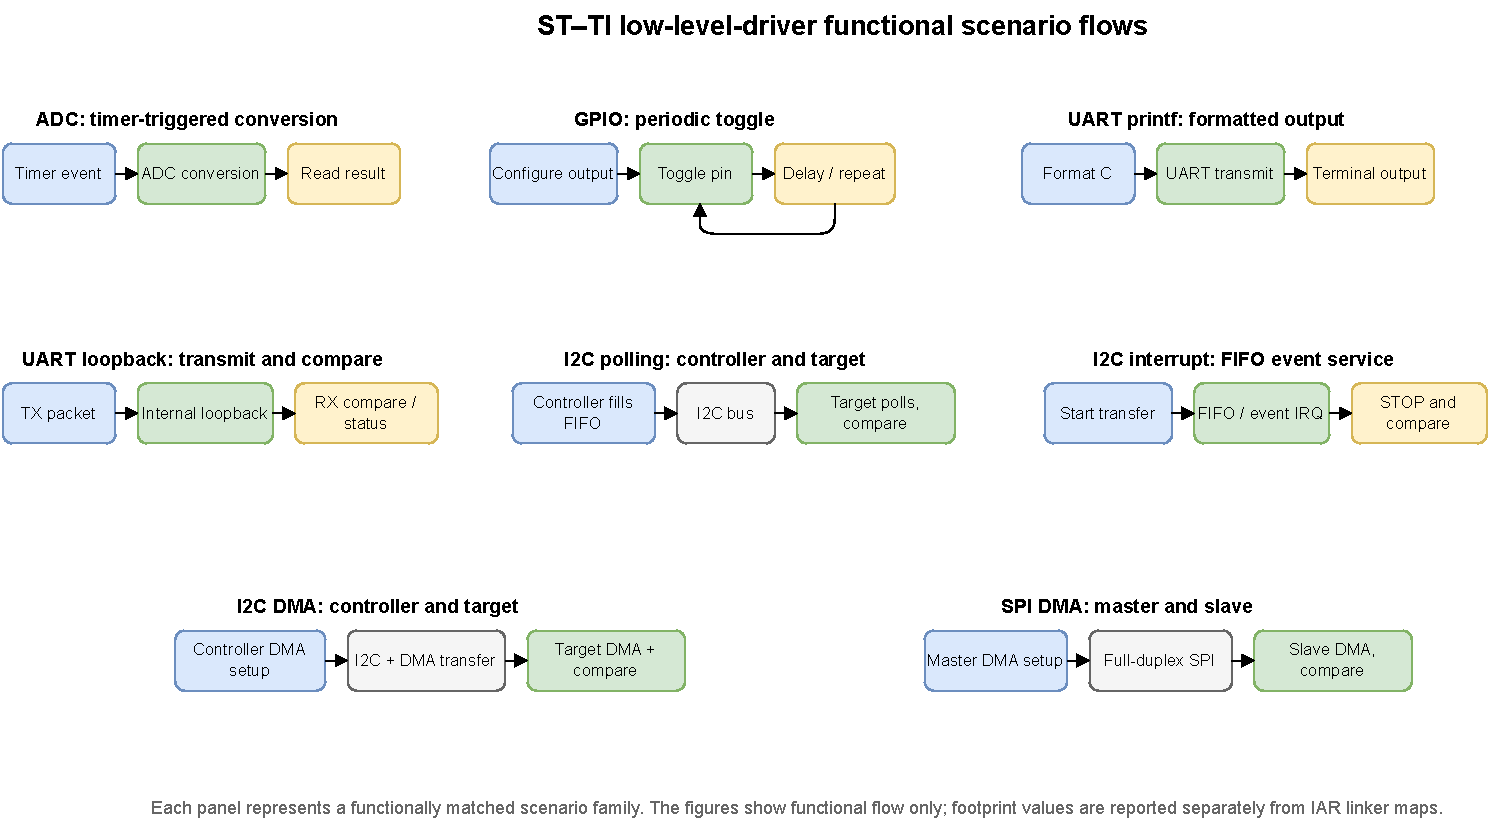
\includegraphics[width=\textwidth]{Figures/ti-functional/scenario-flows.pdf}
\caption{Functional flows of the eight low-level-driver scenario families. I\textsuperscript{2}C and SPI panels represent their paired controller/target and master/slave projects, respectively; the flows define functional behaviour and not a timing window.}
\label{fig:ti-functional-scenario-flows}
\end{figure}

\begin{table}[H]
\centering
\small
\caption{ST--TI low-level-driver functional scenario mapping.}
\label{tab:ti-functional-scenarios}
\begin{tabularx}{\textwidth}{c l X X}
\toprule
\textbf{ID} & \textbf{Scenario} & \textbf{TI driverlib example} & \textbf{STM32CubeC5 LL example} \\
\midrule
1 & ADC, timer-triggered conversion & ADC single conversion & ADC single conversion \\
2 & GPIO output toggle & GPIO I/O toggling & GPIO toggle \\
3 & I\textsuperscript{2}C controller transmit, DMA & I2C two-board DMA, controller & I2C DMA, controller \\
4 & I\textsuperscript{2}C target receive, DMA & I2C two-board DMA, target & I2C DMA, responder \\
5 & I\textsuperscript{2}C controller transmit, interrupt & I2C two-board interrupt, controller & I2C interrupt, controller \\
6 & I\textsuperscript{2}C target receive, interrupt & I2C two-board interrupt, target & I2C interrupt, responder \\
7 & I\textsuperscript{2}C controller transmit, polling & I2C two-board polling, controller & I2C polling, controller \\
8 & I\textsuperscript{2}C target receive, polling & I2C two-board polling, target & I2C polling, responder \\
9 & SPI controller/master full-duplex, DMA & SPI two-board DMA, controller & SPI DMA, master \\
10 & SPI peripheral/slave full-duplex, DMA & SPI two-board DMA, peripheral & SPI DMA, slave \\
11 & UART internal loopback & USART loopback & USART loopback \\
12 & UART formatted output & UART printf & USART printf \\
\bottomrule
\end{tabularx}
\end{table}

\reportscreenshot
      {Figures/ti-functional/screenshots/functional-build-and-map.png}
      {Open one matched TI and ST scenario pair in IAR EWARM. Capture successful build summaries and the corresponding linker-map totals for RO code, RO data, and RW data.}
      {Matched functional scenario builds and linker-map memory totals in IAR EWARM.}
      {fig:ti-screenshot-functional-build}

The I\textsuperscript{2}C and SPI examples validate the transfer path by comparing received
and expected buffers; a successful completion is indicated by the normal LED state, whereas an
error enters the example's error indication path. The UART loopback scenario similarly checks
two four-byte packets. In the formatted-output scenario, both implementations emit the same
single-character payload, \texttt{C}. The ADC and GPIO scenarios provide a conversion value or
a visible pin state, respectively. Figure~\ref{fig:ti-functional-scenario-flows} gives the
functional flow for each scenario family. These observables establish a functional pass/fail
contract; they are separate from execution-time and energy measurements.

\subsection{Results and interpretation}
\label{subsec:ti-functional-results}

The functional projects were rebuilt with IAR EWARM 9.60.3 using high optimisation configured
for size on both platforms. We extracted read-only code, read-only data, and read-write data
from the linker maps, whose memory accounting is documented by IAR~\cite{iar-ewarm}. We define
flash as the sum of read-only code and read-only data, and RAM as read-write data. The latter
includes the linker-reserved stack; both implementations reserve 512 bytes per image,
preserving a common RAM baseline. The results therefore describe complete linked images,
including startup and vector-table costs, rather than only application source files.

Table~\ref{tab:ti-functional-footprint} reports the twelve matched pairs. A negative delta
means that STM32C5 uses less memory. STM32C5 has the smaller flash image in the ADC scenario,
both I\textsuperscript{2}C DMA roles, both I\textsuperscript{2}C polling roles, and the two
UART scenarios. MSPM33 has the smaller flash image for GPIO, both interrupt-driven I\textsuperscript{2}C
roles, and both SPI DMA roles. STM32C5 uses less RAM in every I\textsuperscript{2}C and SPI
pair, while the small ADC, GPIO, and UART examples are equal in RAM.

\begin{table}[H]
\centering
\scriptsize
\caption{Whole-image footprint results from IAR high/size linker maps (bytes). Flash is RO code plus RO data and RAM is RW data~\cite{iar-ewarm}; negative deltas favour STM32C5.}
\label{tab:ti-functional-footprint}
\resizebox{\textwidth}{!}{%
\begin{tabular}{l r r r r r r}
\toprule
\textbf{Scenario} & \textbf{MSPM33 flash} & \textbf{STM32 flash} & \textbf{Flash delta} & \textbf{MSPM33 RAM} & \textbf{STM32 RAM} & \textbf{RAM delta} \\
\midrule
ADC timer trigger & 1\,476 & 1\,416 & -60 (-4.1\%) & 513 & 513 & 0 (0.0\%) \\
GPIO toggle & 656 & 772 & +116 (+17.7\%) & 512 & 512 & 0 (0.0\%) \\
I\textsuperscript{2}C DMA controller & 1\,928 & 1\,840 & -88 (-4.6\%) & 553 & 517 & -36 (-6.5\%) \\
I\textsuperscript{2}C DMA responder & 1\,744 & 1\,687 & -57 (-3.3\%) & 593 & 556 & -37 (-6.2\%) \\
I\textsuperscript{2}C interrupt controller & 1\,580 & 1\,732 & +152 (+9.6\%) & 557 & 514 & -43 (-7.7\%) \\
I\textsuperscript{2}C interrupt responder & 1\,388 & 1\,460 & +72 (+5.2\%) & 600 & 553 & -47 (-7.8\%) \\
I\textsuperscript{2}C polling controller & 1\,420 & 1\,376 & -44 (-3.1\%) & 556 & 513 & -43 (-7.7\%) \\
I\textsuperscript{2}C polling responder & 1\,412 & 1\,340 & -72 (-5.1\%) & 608 & 552 & -56 (-9.2\%) \\
SPI DMA controller & 1\,704 & 2\,151 & +447 (+26.2\%) & 592 & 556 & -36 (-6.1\%) \\
SPI DMA peripheral & 1\,876 & 1\,940 & +64 (+3.4\%) & 592 & 552 & -40 (-6.8\%) \\
UART printf & 1\,326 & 1\,318 & -8 (-0.6\%) & 512 & 512 & 0 (0.0\%) \\
USART loopback & 1\,588 & 1\,580 & -8 (-0.5\%) & 532 & 532 & 0 (0.0\%) \\
\midrule
\textbf{Total, 12 independent images} & \textbf{18\,098} & \textbf{18\,612} & \textbf{+514 (+2.8\%)} & \textbf{6\,720} & \textbf{6\,382} & \textbf{-338 (-5.0\%)} \\
\bottomrule
\end{tabular}%
}
\end{table}

The aggregate must be interpreted as a portfolio sum, not the memory requirement of one
deployable firmware image. Across the twelve independently linked projects, MSPM33 has the
smaller aggregate flash footprint by 514 bytes (2.8\%), whereas STM32C5 has the smaller
aggregate RAM allocation by 338 bytes (5.0\%). The small 8-byte flash differences in UART
printf and loopback are near ties and should not be interpreted as an architectural advantage.

The map attribution explains the mixed flash result. STM32C5 typically carries a larger fixed
startup and vector-table contribution: approximately 460 bytes of read-only data against
276 bytes on MSPM33. GPIO makes this effect visible: STM32C5 uses less read-only code
(312 versus 380 bytes), yet its complete image is 116 bytes larger because the fixed
read-only-data cost dominates the minimal application. In the DMA and polling I\textsuperscript{2}C
scenarios, the STM32 application removes unused buffers, generic initialisation, and inactive
state, so its scenario-specific savings exceed this fixed cost. Interrupt-driven I\textsuperscript{2}C
retains event and error handlers, leaving MSPM33 ahead in flash but STM32C5 ahead in RAM.

SPI DMA controller is STM32C5's largest flash loss, at 447 bytes. The result is not explained
solely by the vector table: the STM32 application explicitly owns GPIO, DMA, SPI, NVIC,
end-of-transfer and DMA-error handling, buffer comparison, LED feedback, and delay behaviour,
whereas the TI project resolves more configuration through SysConfig and DriverLib. This is a
valid whole-SDK implementation result; it does not establish that STM32 hardware intrinsically
requires 447 additional bytes for SPI DMA. Conversely, the smaller STM32 RAM totals arise
primarily from fewer persistent buffers and state variables, not from a smaller stack, whose
512-byte reservation is equal on both sides.

These footprint results are independent of runtime performance. No timing, energy, or
hardware-success conclusion is inferred from linker maps. In particular, I\textsuperscript{2}C
runtime equivalence still requires evidence of matching address acknowledgement, 37-byte
transfer completion, STOP behaviour, target comparison, and identical error handling.

Table~\ref{tab:ti-functional-controls} defines the controls required before publishing runtime
results. It separates the established footprint evidence from platform and measurement
conditions that must be normalised. This distinction is especially important for the ADC
scenario: the TI example stops after a timer-triggered conversion for debugger inspection,
while the ST example continuously reads and transmits conversion values. Those reporting
behaviours must be removed from the timing boundary or made equivalent.

\begin{table}[H]
\centering
\caption{Controls required before quantitative ST--TI functional results are compared.}
\label{tab:ti-functional-controls}
\begin{tabularx}{\textwidth}{l X X}
\toprule
\textbf{Control} & \textbf{Current observation} & \textbf{Required action} \\
\midrule
TI target device & The footprint maps target MSPM33C321A, paired with STM32C5A3ZG. & Record the exact device configuration again in every future runtime result. \\
Core and clock & Footprint does not establish matched runtime clock settings. & Record and normalise core clock, peripheral clock, and timer source for every pair. \\
Build configuration & Debug artifacts and optimisation-labelled example folders coexist. & Build both sides with documented, matched compiler and linker options. \\
Peripheral protocol & Payload length, bus speed, ADC input, and sampling settings are not fully matched. & Set identical functional parameters and preserve them in the scenario configuration. \\
Measurement boundary & LEDs, buttons, UART output, and debugger stops are present in examples. & Measure from the common trigger to verified completion, excluding setup and reporting. \\
Sampling protocol & No repetition count, warm-up policy, or aggregation is implemented. & Capture repeated samples and report the statistic, dispersion, and pass/fail rate. \\
\bottomrule
\end{tabularx}
\end{table}

Once these controls are resolved, each row of Table~\ref{tab:ti-functional-scenarios} can
produce a directly comparable result set: functional pass/fail status, code and data footprint
from matched linker maps, and a normalised timing or energy metric. Until then, the evidence
supports the conclusion that the two libraries cover comparable low-level behaviours across
the selected scenarios, not that one implementation is faster or smaller.

% ====================================================================
\section{FreeRTOS middleware benchmark}
\label{sec:ti-freertos}

The low-level-driver benchmark measures isolated peripheral integrations; it does not exercise
the scheduler and kernel services that structure a concurrent embedded application. We therefore
extended the functional comparison to FreeRTOS~\cite{freertos} using the same three scenario
families introduced in Section~\ref{sec:gd32-freertos}: basic processing, cooperative yielding,
and priority-driven preemption. Project manifests identify FreeRTOS Kernel~V11.2.0 in the
STM32CubeC5 projects and V11.1.0 in the MSPM33 SDK~1.04.00.00 projects; the vendor packages
provide the corresponding source baselines~\cite{freertos-v11,stm32cubec5-sw,ti-mspm33-sdk}.
This version difference is retained as a fairness limitation.

\subsection{Scenario design and configuration}
\label{subsec:ti-freertos-design}

All scenarios use the native FreeRTOS API, a 1\,kHz tick, preemption enabled, time slicing
disabled, dynamic allocation, ten priority levels, and an 8\,KiB FreeRTOS heap. Worker stack
depth is 128 FreeRTOS stack units and the reporter depth is 512 units. Every reporter delays for
30\,s before capturing the cumulative counters and transmitting the observation through a
115200-baud UART. Figure~\ref{fig:ti-freertos-architecture} summarises the task topology.

\begin{figure}[H]
\centering
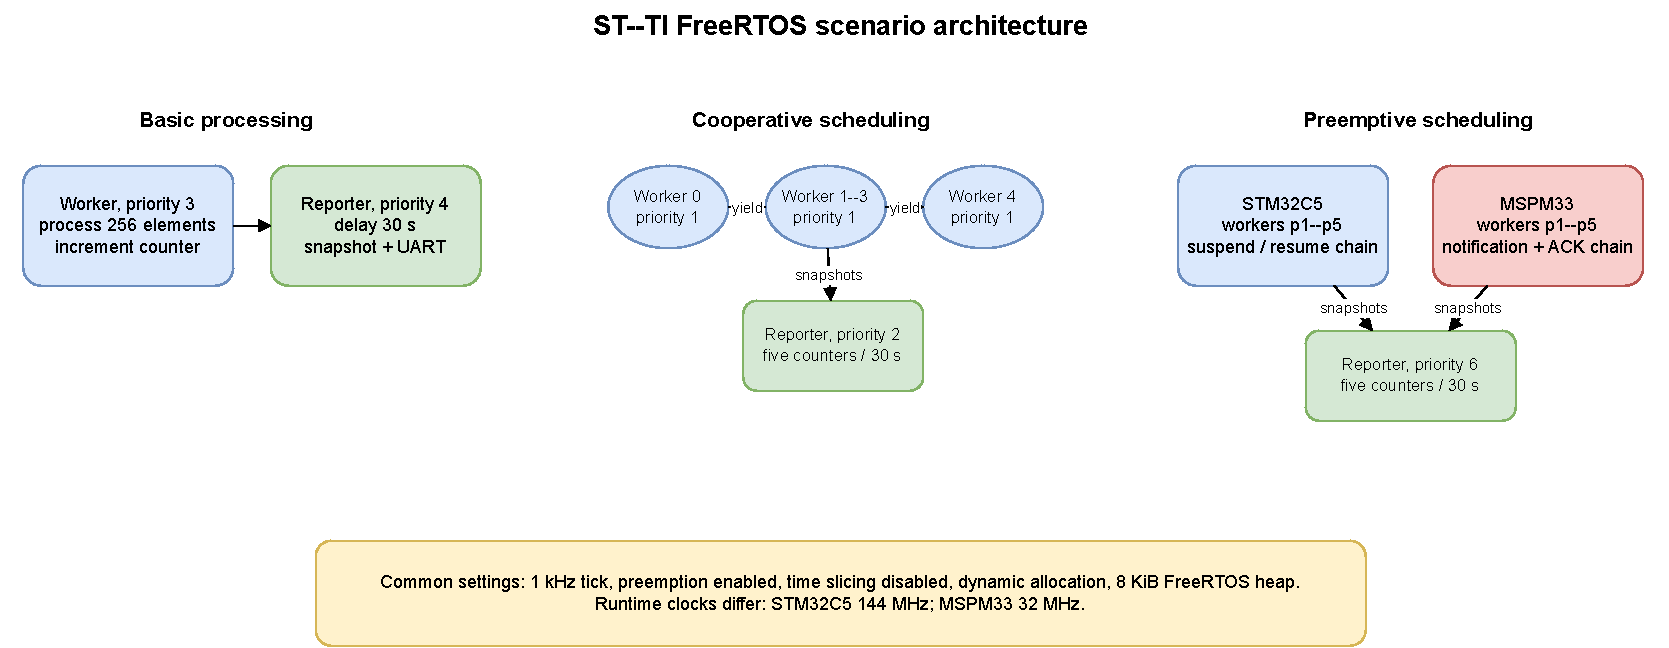
\includegraphics[width=\textwidth]{Figures/ti-freertos/scenario-architecture.pdf}
\caption{Task architecture of the three ST--TI FreeRTOS scenarios. The preemptive scenario deliberately shows the non-equivalent synchronisation paths found in the measured projects.}
\label{fig:ti-freertos-architecture}
\end{figure}

\begin{table}[H]
\centering
\caption{FreeRTOS scenario semantics and reported metric.}
\label{tab:ti-freertos-scenarios}
\begin{tabularx}{\textwidth}{l X X}
\toprule
\textbf{Scenario} & \textbf{Task behaviour} & \textbf{Reported metric} \\
\midrule
Basic & One priority-3 worker transforms a 256-element volatile array and increments a counter; a priority-4 reporter samples it. & Completed processing iterations/s \\
Cooperative & Five priority-1 workers call \texttt{taskYIELD()} and increment separate counters; a priority-2 reporter samples all five. & Mean iterations/thread/s \\
Preemptive & Five workers use priorities 1--5 and a priority-6 reporter. STM32 uses a suspend/resume chain; TI uses task notifications and an acknowledgement. & Mean completed chains/thread/s \\
\bottomrule
\end{tabularx}
\end{table}

The basic and cooperative scenarios preserve the same worker count, creation order, priorities,
and counter semantics on both platforms. The preemptive projects do not preserve the same
synchronisation primitive: STM32 uses \texttt{vTaskSuspend()} and \texttt{vTaskResume()}, while
TI uses direct task notifications plus a final acknowledgement. Its result therefore compares
the two complete implementations but cannot isolate the cost of a common preemption mechanism.

\subsection{Measurement method and fairness}
\label{subsec:ti-freertos-method}

Runtime values were obtained from UART captures supplied after executing both boards. Each row
in Table~\ref{tab:ti-freertos-runtime} is the mean of the available 30-second windows: three
STM32 and two TI windows for basic processing, two and four for cooperative processing, and two
and six for preemptive processing. No warm-up interval or dispersion statistic was recorded.
Cooperative and preemptive reporters advance a nominal time by 30\,s; because UART output occurs
before the next delay, reporting time is outside their denominator.

The largest fairness difference is the configured core clock: STM32C5 runs at 144\,MHz with
instruction cache enabled, whereas MSPM33 runs at 32\,MHz. Both targets use a Cortex-M33 and
Virtual Floating-Point version~5 (VFPv5) single-precision configuration, but the clock ratio is
4.5:1. We therefore report the raw rates and a clock-normalised ratio

\[
R_{\mathrm{norm}} = \frac{R_{\mathrm{STM32}}/144}{R_{\mathrm{MSPM33}}/32}.
\]

A value near one indicates that the raw difference is explained approximately by configured
clock frequency; it is not a direct measurement of cycles per context switch.

\subsection{Results}
\label{subsec:ti-freertos-results}

\begin{table}[H]
\centering
\caption{Observed FreeRTOS runtime rates and clock-normalised STM32/MSPM33 ratio.}
\label{tab:ti-freertos-runtime}
\begin{tabular}{l r r r}
\toprule
\textbf{Scenario} & \textbf{STM32C5 rate} & \textbf{MSPM33 rate} & $\boldsymbol{R_{\mathrm{norm}}}$ \\
\midrule
Basic processing & 43\,172.93 iterations/s & 9\,570.47 iterations/s & 1.002 \\
Cooperative & 226\,652.76 iterations/thread/s & 35\,783.68 iterations/thread/s & 1.408 \\
Preemptive & 55\,015.52 chains/thread/s & 7\,110.96 chains/thread/s & 1.719 \\
\bottomrule
\end{tabular}
\end{table}

\reportscreenshot
      {Figures/ti-freertos/screenshots/uart-runtime-windows.png}
      {Place the STM32C5 and MSPM33 UART captures side by side. Show the board identity, scenario, raw counters, 30-second reporting window, and enough repeated windows to support the values in the runtime table.}
      {Raw UART reporting windows used for the ST--TI FreeRTOS runtime comparison.}
      {fig:ti-screenshot-freertos-uart}

Basic processing scales almost exactly with the configured clock ratio: after normalisation,
STM32C5 and MSPM33 differ by only 0.2\%. The cooperative observation retains a normalised ratio
of 1.408, but this value includes the complete worker loop, FreeRTOS port, compiler runtime,
cache and memory behaviour; it does not measure \texttt{taskYIELD()} in isolation. The
preemptive ratio is larger still, but the different kernel versions and synchronisation
primitives prevent attribution to scheduler efficiency. One TI cooperative run printed
\texttt{ERROR} because the shared integer-truncated balance check allowed only a one-count
deviation; the individual counters remained within the observed scheduling pattern, so this is
treated as a benchmark-check limitation rather than a demonstrated kernel failure.

All six images were rebuilt with IAR EWARM~9.60.3 using high optimisation for size. The
recorded options are \texttt{CCOptLevel=3} and \texttt{CCOptStrategy=1}. Flash is read-only
code plus read-only data; RAM is read-write data, following the linker-map accounting used in
Section~\ref{subsec:ti-functional-results}~\cite{iar-ewarm}.

\begin{table}[H]
\centering
\caption{FreeRTOS whole-image footprint under IAR high/size optimisation (bytes).}
\label{tab:ti-freertos-footprint}
\resizebox{\textwidth}{!}{%
\begin{tabular}{l r r r r r r}
\toprule
& \multicolumn{3}{c}{\textbf{Flash}} & \multicolumn{3}{c}{\textbf{RAM}} \\
\cmidrule(lr){2-4}\cmidrule(lr){5-7}
\textbf{Scenario} & \textbf{STM32} & \textbf{TI} & \textbf{ST--TI} & \textbf{STM32} & \textbf{TI} & \textbf{ST--TI} \\
\midrule
Basic & 9\,052 & 12\,854 & -3\,802 (-29.6\%) & 10\,196 & 10\,140 & +56 (+0.6\%) \\
Cooperative & 9\,640 & 13\,430 & -3\,790 (-28.2\%) & 9\,188 & 9\,132 & +56 (+0.6\%) \\
Preemptive & 10\,012 & 13\,894 & -3\,882 (-27.9\%) & 9\,188 & 9\,112 & +76 (+0.8\%) \\
\midrule
\textbf{Total} & \textbf{28\,704} & \textbf{40\,178} & \textbf{-11\,474 (-28.6\%)} & \textbf{28\,572} & \textbf{28\,384} & \textbf{+188 (+0.7\%)} \\
\bottomrule
\end{tabular}
}
\end{table}

Unlike the low-level-driver portfolio, the middleware result consistently favours STM32C5 in
flash: its three images are 27.9--29.6\% smaller, for an aggregate reduction of 11\,474 bytes.
TI uses slightly less RAM in every scenario, but the difference is only 56--76 bytes per image.
These totals include each platform's complete startup, configuration, C runtime, FreeRTOS
kernel/port, application, heap, and stack reservations. TI links an externally built FreeRTOS
library, while STM32 compiles the kernel sources in each project; configuration also differs in
task notifications, stack-overflow checking, application task tags, and thread-local-storage
pointers. The footprint gap is consequently a result for these deployable SDK configurations,
not a kernel-only size comparison.

Appendix~\ref{sec:appendix-ti-freertos} preserves the raw UART windows, project configuration,
primitive mapping, and linker-map totals used for these calculations.

\subsection{Takeaway}
\label{subsec:ti-freertos-takeaway}

The FreeRTOS benchmark adds two findings to the ST--TI comparison. First, the STM32C5 projects
produce substantially smaller linked flash images while MSPM33 retains a marginal RAM
advantage. Second, raw runtime rates cannot be read as a direct platform ranking: the basic
scenario is almost entirely explained by the 4.5:1 clock ratio, and the more complex scenarios
retain differences that are confounded by kernel configuration and, for preemption, different
synchronisation semantics. A controlled follow-up should use equal clocks, one FreeRTOS version
and configuration, equal primitives, equal sample counts, a warm-up policy, and cycle-level
measurement boundaries.


\newpage
\section*{Conclusion}
This chapter presented the ST-versus-TI comparison of the STM32CubeC5 LL layer and TI
driverlib. The static phase covered seven quality dimensions and an SDK inventory comparison
for the selected releases. The functional phase then mapped twelve bare-metal scenarios spanning ADC, GPIO,
I\textsuperscript{2}C, SPI, and UART behaviour, and documented their observable completion
criteria.

Within the analysed source sets, STM32CubeC5 records higher measured documentation coverage,
lower duplication and average cyclomatic complexity, and a lower adjusted Cppcheck
MISRA-addon finding count. The SDK inventory also identifies broader ST coverage in several
connectivity and security categories. These findings describe the selected SDK versions and
analysis configuration; they do not establish overall ecosystem maturity, certified MISRA
compliance, runtime performance, or product-level software quality.

TI's analysed driverlib makes wider use of enums and typedefs, while the SDK inventory
identifies distinct analog, post-quantum cryptography, AI, graphics, and automotive
capabilities. These are source-structure, datasheet, and inventory observations rather than
measured advantages in execution time, analog performance, safety, or application
suitability.

The functional phase provides whole-image footprint evidence for both the low-level-driver and
FreeRTOS portfolios. The driver scenarios slightly favour MSPM33 in aggregate flash and STM32C5
in RAM, whereas all three FreeRTOS images favour STM32C5 in flash and MSPM33 by a small RAM
margin. Runtime observations are available for FreeRTOS, but unequal clocks, kernel versions,
configuration options, sample counts, and preemptive primitives limit their interpretation.
The basic result is almost exactly clock-proportional; cooperative and preemptive differences
require a controlled follow-up before they can support scheduler-efficiency conclusions.